% !TeX spellcheck = it_IT

\section{Architetture parallele a Memoria Distribuita}
Possiamo rappresentare l'architettura come un \textbf{grafo} $G$, con un \textbf{nodo per ogni processore} e gli \textbf{archi} rappresentano la \textbf{rete di connessione}. \\

\textbf{Non si ha} più una \textbf{memoria condivisa} e non è nemmeno detto che il processore a cui devo inviare i dati sia collegato al processore che li possiede, l'\textbf{informazione} potrebbe dover \textbf{passare da più "processori router"} prima di arrivare a destinazione.

\paragraph{Caratteristiche:}
\begin{itemize}
	\item \textbf{Processori}: RAM sequenziali, con istruzioni per il calcolo e memoria privata, ma devono anche spedire informazioni (fare da "router"), quindi servono \textbf{istruzioni per la comunicazione}, ovvero \texttt{send} e \texttt{receive}.\\
	Da notare che anche la \textbf{comunicazione avviene in parallelo}, quindi se $n$ processori provano a spedire dati a un solo processore, questo dovrà impiegare $n+1$ passi per ricevere tutto.\\
	
	\item \textbf{Collegamenti}: di tipo Full-duplex, gli archi del grafo sono non diretti, non avrebbe senso avere canali di comunicazione a un solo senso. Due processori collegati, per comunicare tra di loro impiegano 2 passi (tempo costante), cosa non vera per 2 processori più lontani.\\
	
	\item \textbf{Clock centrale}: scandisce il tempo per tutti i processori.\\
	
	\item \textbf{Programma}: come nelle PRAM, ci sono i \texttt{par do} e tutti i processori eseguono la stessa istruzione (SIMD, vedi \hyperref[subsubsec:PRAM]{PRAM}). Come già detto, si aggiungono le istruzioni di \texttt{send} e \texttt{receive}.\\
	
	\item \textbf{Input/Output}: non abbiamo una memoria condivisa, quindi: 
	\begin{itemize}
		\item Input: distribuito tra i processori
		\item Output: o su un processore dedicato, o si legge in un certo ordine tra i vari processori
	\end{itemize}
	\nn
	
	\item \textbf{Risorse di calcolo}
	\begin{itemize}
		\item Numero di processori
		\item Tempo, dato da tempo di calcolo $+$ tempo di comunicazione
	\end{itemize}
\end{itemize}

\newpage

\subsection{Parametri di Rete}

Data l'architettura $G = (V,E)$, \textbf{definiamo}: 
\begin{itemize}
	\item \textbf{Grado} di $G$:
	$$ \gamma = \max \left\{ \rho (v) | v \in V \right\}$$
	dove $\rho (v)$ è il numero di archi incidenti su $v$ (grado). Quindi è il \textbf{grado massimo del grafo}. Un $\gamma$ alto permette buone comunicazioni ma rende più difficile la realizzazione fisica.\\
	
	\item \textbf{Diametro} di $G$: 
	$$ \delta = \max \left\{ d(v,w) | v,w \in V, \; v \neq w \right\}$$
	dove $d(v,w)$ rappresenta la distanza (numero di nodi da attraversare) minima per andare da $v$ a $w$. Il diametro è la \textbf{massima distanza tra 2 nodi}. Valori bassi di $\delta$ sono preferibili, ma aumentano il parametro $\gamma$.\\
	
	\item \textbf{Ampiezza di bisezione} di $G$: si indica con $\beta$ e indica il \textbf{minimo numero di archi} in $G$ che \textbf{tolti dividono i nodi in circa due metà}. Rappresenta la capacità di trasferire le informazioni in $G$, un valore di $\beta$ alto è preferibile ma incrementa $\gamma$.\\
\end{itemize}

% End Videolezione 14

\newpage

\subsection{Tipici problemi} 
Tipici problemi che mettono in \textbf{risalto pregi e difetti} di queste architetture:
\begin{itemize}
	\item \texttt{Max}: massimo, richiede una comunicazione a coppie di processori, quindi è determinato da $\delta$.\\
	
	\item \texttt{Ordinamento}: si richiede lo spostamento di parti dell'input, quindi è determinato da $\beta$.\\
\end{itemize}

\paragraph{Fact I:} Il tempo richiesto per risolvere \texttt{Max} in $G$ è almeno $\delta$. \\
Dimostrazione: Ogni coppia di processori deve comunicare.\\

\paragraph{Fact II:} il tempo richiesto per risolvere l'ordinamento in $G$ è almeno $n/2 \cdot 1/\beta$.\\
Dimostrazione: come minimo devo controllare ed eventualmente scambiare ogni coppia di dati, quindi $n/2$, e posso controllarne parallelamente $\beta$ per volta.\\

Quindi la \textbf{topologia di rete impatta il tempo}
$$ T_{Max} = \Omega (\delta) $$
$$ T_{Ord} = \Omega \left(\frac{n}{2 \beta} \right) $$

\newpage

\subsection{Confrontatori}
Per affrontare i problemi \texttt{Max} e \texttt{Ordinamento} introduciamo i confrontatori e primitive.\\

\paragraph{Definizione:} Istruzioni di confronto per i confrontatori (o comparatori), possono essere:
\begin{itemize}
	\item \texttt{if (A[i] > A[j]) then Swap(A[i], A[j])}
	\item \texttt{if (A[i] < A[j]) then Swap(A[i], A[j])}
\end{itemize}

\begin{center}
	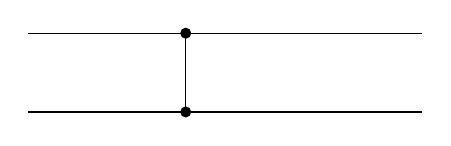
\begin{tikzpicture} % Draw the two parallel lines 
		\draw (0,0) -- (5,0); 
		\draw (0,1) -- (5,1); 
		
		% Draw the connecting line 
		\draw (2,0) -- (2,1);
		
		% Nodes
		\fill (2,0) circle (2pt); 
		\fill (2,1) circle (2pt); 
	\end{tikzpicture}
\end{center}

Sostanzialmente, due fili collegati da un confrontatore il quale mette sopra il minimo e sotto il massimo (o viceversa, in base alla forma).\\

Sono stati definiti per le \textbf{sorting network}, reti di confrontatori che permettono di ordinare $n$ elementi.\\
Esempio a 3 elementi: 
\begin{center}
	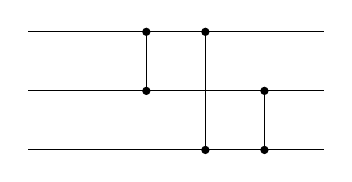
\begin{tikzpicture} [scale=0.75]
		% Draw the two parallel lines 
		\draw (0,0) -- (5,0); 
		\draw (0,1) -- (5,1); 
		\draw (0,2) -- (5,2); 
		
		% Draw the connecting line 
		\draw (2,2) -- (2,1);
		\draw (3,2) -- (3,0);
		\draw (4,1) -- (4,0);
		
		% Nodes
		\fill (2,2) circle (2pt); 
		\fill (2,1) circle (2pt); 
		\fill (3,2) circle (2pt); 
		\fill (3,0) circle (2pt); 
		\fill (4,1) circle (2pt); 
		\fill (4,0) circle (2pt); 
	\end{tikzpicture}
\end{center}

Le sorting network danno ispirazione ad \textbf{algoritmi di ordinamento}: 
\begin{center}
	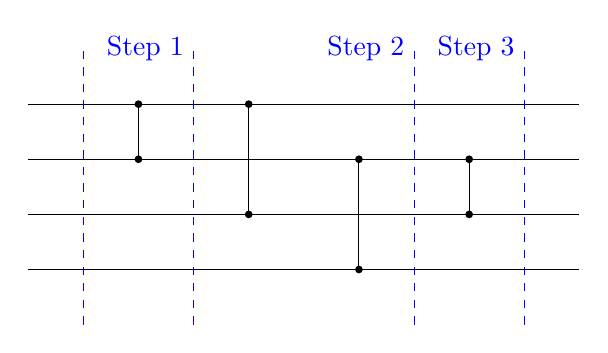
\begin{tikzpicture} [scale=0.7]
		% Draw the two parallel lines 
		\draw (0,0) -- (10,0); 
		\draw (0,1) -- (10,1); 
		\draw (0,2) -- (10,2); 
		\draw (0,3) -- (10,3); 
		
		% Draw the connecting line 
		\draw (2,3) -- (2,2);
		\draw (4,3) -- (4,1);
		\draw (6,2) -- (6,0);
		\draw (8,2) -- (8,1);
		
		\draw[dashed, blue] (1,-1) -- (1,4) node[left] {};
		\draw[dashed, blue] (3,-1) -- (3,4) node[left] {Step 1};
		\draw[dashed, blue] (7,-1) -- (7,4) node[left] {Step 2};
		\draw[dashed, blue] (9,-1) -- (9,4) node[left] {Step 3};
		
		% Nodes
		\fill (2,3) circle (2pt); 
		\fill (2,2) circle (2pt); 
		\fill (4,3) circle (2pt); 
		\fill (4,1) circle (2pt); 
		\fill (6,2) circle (2pt); 
		\fill (6,0) circle (2pt); 
		\fill (8,2) circle (2pt); 
		\fill (8,1) circle (2pt); 
	\end{tikzpicture}
\end{center}

\newpage

Si può assegnare ad ogni linea un processore ed uno step è il massimo insieme contiguo di confrontatori che occupano ogni confrontatore al più una volta sola, senza rompere la sequenza di esecuzione (da formalizzare un po').\\

Quindi per l'esempio sopra:
$$ T(n) = \# \text{ Step } = 3, \;\;\;\; p(n) = \# \text{ Fili } = 4 $$

Formalizziamo una \textbf{rete di confrontatori} come: 
$$ R (x_1, \, \dots \, , x_n) = (y_1, \, \dots \, , y_n) $$

dove $(x_1, \, \dots \, , x_n)$ rappresenta gli $n$ input e $(y_1, \, \dots \, , y_n)$ gli $n$ output.\\

Si dice che $R$ è una \textbf{sorting network iff} $\forall (x_1, \, \dots \, , x_n) \in \mathbb{N}$ vale 
$$ R (x_1, \, \dots \, , x_n) = (y_1, \, \dots \, , y_n) \; \text{ con } \; y_1 < \, \dots \, < y_n $$
ovviamente l'output deve essere una permutazione dell'input.\\

Dette anche reti di ordinamento "\textit{oblivious}", non dipende dall'input, la rete è ignara di ciò che ci passa sopra.\\

\newpage

\subsubsection{Valutare una rete}

Per capire se \textbf{una rete è una sorting network} si può usare il principio $0$-$1$.\\

Formalmente, è una sorting network se: 
\begin{itemize}
	\item $\forall x \in \{0,1\}^n$, $R(x)$ è ordinato\\
	$\implies \forall x \in \mathbb{N}^n$ si ha $R(x)$ è ordinato.\\
\end{itemize}

Il che è equivalente a dire che:
\begin{itemize}
	\item $\exists x \in \mathbb{N}^n$ tale che $R(x)$ non è ordinato\\
	$\implies \exists x \in \{0,1\}^n$ tale che $R(x)$ non è ordinato.\\
\end{itemize}

Se ordina bene vettori booleani allora ordina bene anche vettori di naturali, quindi posso valutare la rete solo su vettori booleani.\\

\paragraph{$f$-shift:} Prima di applicare la rete $R$ possiamo applicare una funzione $f$ monotona crescente ed è equivalente ad applicare $f$ dopo $R$
$$ R \left(f(x_1), \, \dots \, f(x_n)\right) = \vec{f}\left(R(x_1, \, \dots \, , x_n)\right) = \left(f(y_1), \, \dots \, , f(y_n) \right) $$

Insomma, una funzione monotona crescente posso applicarla sia prima che dopo.\\

\newpage

Ipotizzando di avere una sorting network $R$ \textbf{non corretta}: 
$$ \exists x \in \mathbb{N}^n \; \text{ t.c. } \; R(x) = (y_1, \, \dots \, , y_k, \, \dots \, , y_s, \, \dots \, , y_n)$$

con $y_k > y_s$ e $k<s$ (il vettore non è ordinato per un qualche input $x$).\\

Definiamo una \textbf{funzione} $g: \mathbb{N} \rightarrow \{0,1\}$:
$$ 
g(x) \begin{cases}
	1  & x \geq y_k \\
	0 & \text{altrimenti}
\end{cases}
$$
$g$ è monotona crescente. $y_k$ sarà mappato in $1$ mentre $y_s$ in $0$.\\

Se applico $g$ prima di $R$ ottengo un \textbf{vettore binario} a cui \textbf{applicare la rete}
$$ R\left(g(x_1), \, \dots \, , g(x_n)\right)$$

ma per la regola dello shift diventa uguale a 
$$ = \left(g(y_1), \, \dots \, , g(y_k), \, \dots \, , g(y_s), \, \dots \, , g(y_n) \right)$$

Ma abbiamo $g(y_k) = 1$ prima di $g(y_s) = 0$, di conseguenza \textbf{non ha ordinato il vettore binario}. Ogni vettore naturale può essere trasformato in questo modo.\\

\paragraph{Osservazione:} per capire se $R$ è una sorting network valuto $R$ solo su input binari.\\

% End L15

\newpage

\subsection{Array Lineari}

Gli array lineari sono un'architettura \textbf{parallela} a \textbf{memoria distribuita}, tutti i processori da $P_1$ a $P_n$ sono collegati "in linea", \textbf{ogni processore} è \textbf{collegato} al \textbf{successivo e al precedente}.\\

\textbf{Parametri di rete}: 
\begin{itemize}
	\item \textbf{Grado} $\gamma = 2$, ottimo per la realizzazione, ogni processore è collegato ad altri 2.\\
	
	\item \textbf{Diametro} $\delta = n-1$, lower bound per \texttt{Max} $\delta \sim n$ (non eccezionale, in quanto pari al sequenziale, andrà abbassato), i processori più distanti in assoluto sono $P_1$ e $P_n$ e serve passare $n-1$ collegamenti.\\
	
	\item \textbf{Ampiezza di bisezione} $\beta = 1$, lower bound per Ordinamento $\sfrac{n}{2}$, rappresenta il bottleneck per quanto riguarda l'afflusso dei dati da una metà all'altra dell'architettura.\\
\end{itemize}

Ricordiamo che su PRAM il massimo e ordinamento hanno tempo logaritmico e processori $\sfrac{n}{\log n}$ e $n$ rispettivamente. \\

Negli array lineari è \textbf{necessaria comunicazione}, bisogna quindi aggiungere, come minimo, il tempo necessario per quest'ultima.\\

\newpage

\subsubsection{Primitiva Swap contiguo}

\textbf{Scambiare} i dati in $k$ e $k+1$. Abbiamo due \textbf{processori consecutivi}, quindi collegati direttamente, $P_k$ contiene il dato $A[k]$, $p_{k+1}$ contiene il dato $A[k+1]$ e bisogna scambiarli.\\

Per scambiare i dati:
\begin{center}
	\begin{tabular}{c c}
		$P_k$ & $P_{k+1}$ \\
		\texttt{S} $\rightarrow$ & $\leftarrow$ \texttt{S} \\
		\texttt{R} $\leftarrow$ & $\rightarrow$ \texttt{R} \\
		$A[k] = A[k+1]$ & $A[k+1] = A[k]$ \\
	\end{tabular}
\end{center}
Dove \texttt{S} e \texttt{R} indicano i comandi \texttt{send} e \texttt{receive}. \\

Bisogna fare i due \texttt{send}, al passo dopo i due \texttt{receive} e infine lo swap effettivo dei dati. Servono quindi 3 passi paralleli.\\

Quindi il tempo è costante, dato che i processori sono collegati tra loro, altrimenti bisognerebbe considerare la distanza tra i processori.\\

\newpage

\subsection{Problema Shuffle}

In \textbf{input} un vettore di lunghezza pari, in \textbf{output} la prima metà dell'input innestata dalla seconda metà.\\

\textbf{Idea}: 
\begin{center}
	\begin{tabular}{c c c c c c c c}
		Input: & \texttt{A[1]} & \texttt{A[2]} & \dots & \texttt{A[S]} & \texttt{A[S+1]} & \dots & \texttt{A[2S]} \\
		Output: & \texttt{A[1]} & \texttt{A[S+1]} & \texttt{A[2]} & \texttt{A[S+2]} & \dots & \texttt{A[S]} & \texttt{A[2S]} \\
	\end{tabular}
\end{center}

Questo problema si può risolvere tramite \textbf{swap contigui} tra processori, \textbf{partendo dal centro}, creando una sorta di albero di swap contigui, scambiando elementi fino a portarli nella posizione corretta, con numero di scambi crescente fino a raggiungere le estremità dell'array.\\

\paragraph{Prestazioni:}
\begin{itemize}
	\item \textbf{Processori}: non bisogna arrivare all'estremità quindi ne basta uno in meno, ma comunque lineare
	$$ p = 2(S-1)$$
	
	\item \textbf{Tempo}: il numero di passi è $S-1$, più il costo dello swap, comunque lineare
	$$ t = 3(S-1) $$
	
	\item \textbf{Efficienza}: considerando che lo shuffle sequenziale (senza memoria aggiuntiva) richiede $\Theta (S^2)$, abbiamo
	$$ E \sim \frac{S^2}{S \cdot S} = c \neq 0 $$ 
	quindi è un buon algoritmo.\\
\end{itemize}

\newpage

\subsection{Trasmettere Dati}

Visto che i \textbf{dati} sono \textbf{distribuiti} tra le memorie private dei processori, servirà un'istruzione per spedirli. Ci sarà una \textbf{richiesta di spedizione} del dato $A[i]$ contenuto in $P_i$ verso il processore $P_j$. \\

Definiamo la \textbf{primitiva} \texttt{SEND(i,j)}, dove $i$ è l'indice del processore che spedisce e $j$ del recipiente. Entra in gioco la distanza tra i due processori, dovendo seguire un cammino da $P_i$ a $P_j$ all'interno dell'architettura.\\

Per \textbf{inviare i dati}: 
\begin{itemize}
	\item $P_i$ fa una \texttt{Send} verso $P_{i+1}$
	\item $P_{i+1}$ fa una \texttt{Receive} ed una \texttt{Send} verso il processore successivo
	\item Si \textbf{ripete} fino ad arrivare a $P_j$ che farà solo una \texttt{Receive}
\end{itemize}

In \textbf{totale} si hanno $2 d(i,j)$ \textbf{passi paralleli}, dove $d(i,j)$ è la distanza tra $P_i$ e $P_j$. Il \textbf{costo di trasmissione} per un dato in un array lineare è sempre 2 volte la distanza tra i processori.\\

La trasmissione \textbf{non è costante} come nella PRAM.\\

\newpage

\subsection{Problema \texttt{Max}}
Vogliamo calcolare il \textbf{massimo} tra $n$ elementi in input.\\

\textbf{Definizione}: 
\begin{itemize}
	\item \textbf{Input}: \texttt{A[1] A[2] \dots \; A[n]}, $n$ valori
	\item \textbf{Output}: $cont(P_n) = \max\{A[i] | 1 \leq i \leq n\}$, ovvero il contenuto del processore con indice più alto deve essere il massimo tra tutti i valori
\end{itemize}

Il \textbf{tempo} per \texttt{Max} su array lineari è \textbf{limitato inferiormente da} $n$ (su PRAM è $\log n$, su sequenziale è $n$).\\

\textbf{Idea} dell'algoritmo: 
\begin{itemize}
	\item Considerando l'algoritmo per sommatoria su PRAM (dato che vale per ogni operazione associativa)
	\item Riduzione dei passi per abbassate $\Omega (n)$ su array ad $n$ processori
\end{itemize}

Esempio: $P_1$ invia a $P_2$ il valore e quest'ultimo calcola il massimo, stessa cosa con $P_3$ e $P_4$ e così via; al passaggio dopo $P_2$ invia a $P_4$, $P_6$ a $P_8$ e si continuo fino al massimo globale.\\

\begin{center}
	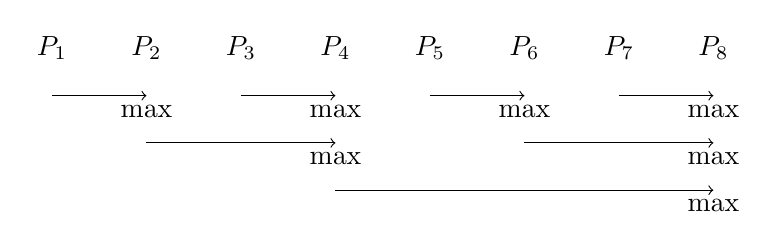
\begin{tikzpicture}[scale=0.6]
		\node (1) at (0,0) {$P_1$};
		\node (2) at (2,0) {$P_2$};
		\node (3) at (4,0) {$P_3$};
		\node (4) at (6,0) {$P_4$};
		\node (5) at (8,0) {$P_5$};
		\node (6) at (10,0) {$P_6$};
		\node (7) at (12,0) {$P_7$};
		\node (8) at (14,0) {$P_8$};
		
		\draw[->] (0,-1) -- (2,-1) node[below] {max};
		\draw[->] (4,-1) -- (6,-1) node[below] {max};
		\draw[->] (8,-1) -- (10,-1) node[below] {max};
		\draw[->] (12,-1) -- (14,-1) node[below] {max};
		
		\draw[->] (2,-2) -- (6,-2) node[below] {max};
		\draw[->] (10,-2) -- (14,-2) node[below] {max};
		
		\draw[->] (6,-3) -- (14,-3) node[below] {max};
	\end{tikzpicture}
\end{center}

Ogni riga un passaggio.\\

\newpage

\textbf{Procedimento}: al $j$-esimo passo ogni processore si confronta con i valori contenuti a distanza $2^{j-1}$ e il risultato viene memorizzato nel processore di indice $2^j \cdot t$. Per il passaggio $j$-esimo si ha il confronto tra i processori $2^{j}t - 2^{j-1}$ e $2^{j}t$, memorizzando il risultato del calcolo in quest'ultimo, per ogni $t \in [1, \sfrac{n}{2^j}]$.\\

Il \textbf{numero di passi} è $\log n$, in quanto confronto a distanza doppia a ogni passo.\\

\textbf{Codice}: 
\begin{lstlisting}[escapeinside={(*}{*)}]
	for (*$j=1$*) to (*$\log n$*)
		for (*$k \in \{2^j t - 2^{j-1} | 1 \leq t \leq \sfrac{n}{2^j}\}$*) par do
			Send((*$k$*), (*$k + 2^{j-1}$*))
		for (*$k \in \{2^j t | 1 \leq t \leq \sfrac{n}{2^j}\}$*) par do
			if (A[(*$k$*) < (*$k - 2^{j-1}$*)]) then 
				A[(*$k$*)] = A[(*$k-2^{j-1}$*)]
\end{lstlisting}

Si possono vedere \textbf{due fasi}, una in cui vengono inviati i dati (con il \texttt{Send}) e una seconda in cui viene effettuato il \texttt{Compare}.\\

\paragraph{Prestazioni:}
\begin{itemize}
	\item \textbf{Tempo}: dobbiamo considerare le due fasi
	\begin{itemize}
		\item per la fase di \texttt{Send} il costo è $2 \cdot 2^{j-1}$, per ogni $j = 1, \, \dots \, , \log n$
		\item per la fase di \texttt{Compare} il costo è $2$, per ogni $j = 1, \, \dots \,, \log n$
	\end{itemize}
	In totale
	$$ t = \sum_{j=1}^{\log n} 2 \cdot s^{j-1} + \sum_{j=1}^{\log n} 2 = 2n-2 + 2 \log n = O(n) $$
	\nn
	
	\item \textbf{Processori}: ne usa $n$, ma non va troppo bene, $E \rightarrow 0$.\\
\end{itemize}

\newpage

\textbf{Riduciamo} i \textbf{processori} da $n$ a $p$, \textbf{riducendo} la \textbf{distanza} $\delta$ e facendo in modo che ogni processore avrà $n/p$ elementi al suo interno. \\

Quindi \textbf{ogni processore} farà il \texttt{Max} sequenziale tra i suoi $n/p$ numeri e poi si esegue il \texttt{Max} \textbf{parallelo} su $p$ \textbf{processori}. \\

Nuove \textbf{prestazioni}: 
\begin{itemize}
	\item \textbf{Processori}: 
	$$ n = p$$
	
	\item \textbf{Tempo}:
	$$ t = O\left(\frac{n}{p}\right) + O(p)$$
	
	\item \textbf{Efficienza}:
	$$ E = \frac{n}{ p \cdot \left(O\left(\frac{n}{p}\right) + O(p)\right)} = \frac{n}{O(n) + O(p^2)}$$
	
	Volendo $O(n)$ al denominatore, per avere $E \rightarrow c \neq 0$ scelgo 
	$$p^2 = n \implies p = \sqrt{n}$$
	\nn
\end{itemize}

Di conseguenza: \texttt{Max} è risolto in modo \textbf{efficiente} su \textbf{array lineari con}
$$ p = \sqrt{n} \; \text{ e } \; T = O \left(\frac{n}{\sqrt{n}}\right) + O(\sqrt{n}) = O(\sqrt{n}) $$

\newpage

\subsection{Swap Non Contiguo}

Generalizziamo l'operazione dello \texttt{Swap} contiguo a processori non vicini.\\

Le connessioni sono full duplex, quindi le \texttt{Send} possono essere effettuate simultaneamente. Bisogna distinguere tra due casi, in quanto la distanza tra i processori può essere pari o dispari: 
\begin{itemize}
	\item \textbf{Primo caso}: distanza \textbf{dispari}
	$$ d(i,j) = 2k + 1 $$
	Quindi i processori coinvolti sono pari, sono $2k+2$. Al centro abbiamo i processori $P_{k+i}$ e $P_{k+i+1}$ i quali saranno in tempo per fare due \texttt{Send} simultanee e due \texttt{Receive} simultanee al passaggio successivo. Si "incrociano" i dati e si continua.\\
	
	\textbf{Tempo}: 
	$$ T = 2k + 2 + 2k + 1 = 4k + 3 = 2(2k + 1) + 1 = 2 d(i,j) + 1 $$
	I $2k$ sono dovuti alle \texttt{Send}, il 2 e l'1 sono dovuti, rispettivamente, allo scambio centrale e all'assegnamento finale. In totale diventa il costo delle \texttt{Send} più 1 per l'assegnamento\\
	
	
	\item \textbf{Secondo caso}: distanza \textbf{pari}
	$$ d(i,j) = 2k $$
	Il numero di processori è dispari e ci sarà un processore centrale che deve gestire le due \texttt{Receive} contemporaneamente. Queste richieste andranno gestite sequenzialmente, allungando di 2 operazioni il tempo visto nel caso precedente.\\
	
	\textbf{Tempo}
	$$ T = 2 d(i,j) + 3 $$
\end{itemize}

\newpage

\subsection{Primitiva \texttt{MinMax}}

Vogliamo avere sul processore di indice inferiore il numero più basso.\\

Tra processori contigui basta fare:
\begin{center}
	\begin{tabular}{c c}
		$P_k$ & $P_{k+1}$ \\
		\texttt{Send} & \texttt{Send} \\
		\texttt{Receive} & \texttt{Receive} \\
		\texttt{if (A[k]>A[k+1])} & \texttt{if (A[k]<A[k+1])} \\
		\texttt{A[k] = A[k+1]} & \texttt{A[k+1] = A[k]}
	\end{tabular}
\end{center}

Quindi impiega \textbf{tempo costante} $T = 4$.\\

Si può \textbf{generalizzare} a \texttt{MinMax(i,j)}, sfruttando \texttt{Swap(i,j)} per poi fare il confronto.\\

\textbf{Tempo} per la versione generica: 
\begin{itemize}
	\item Distanza \textbf{pari}: 
	$$ T = 2 d(i,j) + 2 $$
	\item Distanza \textbf{dispari}:
	$$ T = 2 d(i,j) + 4 $$
\end{itemize}

%End L16

\newpage

\subsection{Problema \texttt{Ordinamento}}

Definizione:
\begin{itemize}
	\item \textbf{Input}: \texttt{A[1]  A[2] \dots  \; A[n]}
	\item \textbf{Output}: $cont(P_1) < cont(P_2) < \, \dots \, < cont(P_n)$, permutazione ordinata
\end{itemize} 

Algoritmo \textbf{test/swap oblivious} descritto da una sorting network, chiamata \textbf{\texttt{Odd/Even} sorting network}.\\

\textbf{Esempio} con 6 elementi: 
\begin{center}
	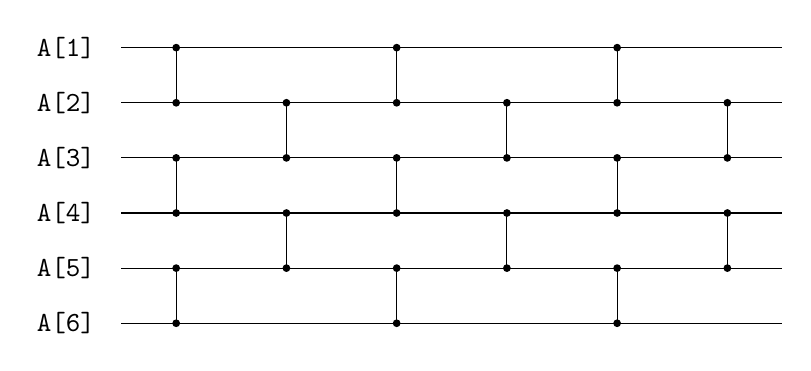
\begin{tikzpicture} [scale=0.7]
		\node (1) at (-1,0) {\texttt{A[6]}};
		\node (1) at (-1,1) {\texttt{A[5]}};
		\node (1) at (-1,2) {\texttt{A[4]}};
		\node (1) at (-1,3) {\texttt{A[3]}};
		\node (1) at (-1,4) {\texttt{A[2]}};
		\node (1) at (-1,5) {\texttt{A[1]}};
		
		% Draw the two parallel lines 
		\draw (0,0) -- (12,0); 
		\draw (0,1) -- (12,1); 
		\draw (0,2) -- (12,2); 
		\draw (0,3) -- (12,3); 
		\draw (0,4) -- (12,4); 
		\draw (0,5) -- (12,5); 
		
		% Draw the connecting line 
		\draw (1,0) -- (1,1);
		\draw (1,2) -- (1,3);
		\draw (1,4) -- (1,5);
		
		\draw (3,1) -- (3,2);
		\draw (3,3) -- (3,4);
		
		\draw (5,0) -- (5,1);
		\draw (5,2) -- (5,3);
		\draw (5,4) -- (5,5);
		
		\draw (7,1) -- (7,2);
		\draw (7,3) -- (7,4);
		
		\draw (9,0) -- (9,1);
		\draw (9,2) -- (9,3);
		\draw (9,4) -- (9,5);
		
		\draw (11,1) -- (11,2);
		\draw (11,3) -- (11,4);
		
		% Nodes
		\fill (1,0) circle (2pt); 
		\fill (1,1) circle (2pt); 
		\fill (1,2) circle (2pt); 
		\fill (1,3) circle (2pt); 
		\fill (1,4) circle (2pt); 
		\fill (1,5) circle (2pt); 
		
		\fill (3,1) circle (2pt); 
		\fill (3,2) circle (2pt); 
		\fill (3,3) circle (2pt); 
		\fill (3,4) circle (2pt); 
		
		\fill (5,0) circle (2pt); 
		\fill (5,1) circle (2pt); 
		\fill (5,2) circle (2pt); 
		\fill (5,3) circle (2pt); 
		\fill (5,4) circle (2pt); 
		\fill (5,5) circle (2pt); 
		
		\fill (7,1) circle (2pt); 
		\fill (7,2) circle (2pt); 
		\fill (7,3) circle (2pt); 
		\fill (7,4) circle (2pt); 
		
		\fill (9,0) circle (2pt); 
		\fill (9,1) circle (2pt); 
		\fill (9,2) circle (2pt); 
		\fill (9,3) circle (2pt); 
		\fill (9,4) circle (2pt); 
		\fill (9,5) circle (2pt); 
		
		\fill (11,1) circle (2pt); 
		\fill (11,2) circle (2pt); 
		\fill (11,3) circle (2pt); 
		\fill (11,4) circle (2pt); 
		
	\end{tikzpicture}
\end{center}

Si alternano \textbf{confrontatori} "\textit{dispari}" con confrontatori "\textit{pari}", per $n$ passaggi.\\

\paragraph{Correttezza:} possiamo usare il principio 0/1, mostrando che l'algoritmo è in grado di \textbf{ordinare qualsiasi vettore binario}:
$$\{0,1\}^n \rightarrow \; \fbox{Odd/Even} \; \rightarrow o^j 1^e  $$

Partendo dal caso peggiore $111100$, $e=4$, $j=2$. Ogni 1 nell'input deve \textbf{scendere} di un \textbf{numero di posizioni} $n-e=j$ (numero di zeri).\\

\textbf{Regola generale}: l'$i$-esimo 1 dal basso, impiega (al più) $n-e+i$ \textbf{passi} per posizionarsi correttamente.\\
Dato che $i \leq e$ si ottiene: $n-e+e = n$, al più $n$ passi.\\

Per quest'algoritmo $n$ \textbf{passi} sono \textbf{necessari e sufficienti}.

\newpage

Implementazione \textbf{sequenziale}: $T(n,1) = O(n^2)$ (sostanzialmente un BubbleSort).\\

\paragraph{Implementazione parallela:} richiede $n$ round di comparatori implementati con \texttt{MinMax(k,k+1)}. \\

\textbf{Codice}: 
\begin{lstlisting}[escapeinside={(*}{*)}]
	for (*$i = 1$*) to (*$n$*)
		for (*$k \in \{ 2t - (i \% 2) | 1 \leq t \leq n/2 \} $*) par do
			MinMax((*$k$*), (*$k+1$*) )
\end{lstlisting}

La condizione del \texttt{for} fa attivare alternativamente processori pari e dispari.\\

\paragraph{Prestazioni: }
\begin{itemize}
	\item \textbf{Tempo}: 
	$$ t = n \cdot 4 = O(n) $$
	\item Numero di \textbf{processori}: 
	$$ p = n $$
	\item \textbf{Efficienza}: 
	$$ E = \frac{n \log n}{n \cdot n} \rightarrow 0 $$
\end{itemize}

\paragraph{Osservazione:} Per $n$ processori in un array lineare l'ordinamento richiede, come \textbf{lower bound}, tempo $\Omega \left(\frac{n}{2 \beta}\right)$, dove $\beta = 1$.\\

\newpage

\subsubsection{Merge-Split}

\textbf{Riduzione} dei \textbf{processori}: Al posto di usarne $n$ ne \textbf{usiamo} $p$.\\

Ogni processore conterrà $n/p$ dati e li \textbf{ordina sequenzialmente} in un \textbf{tempo} 
$$ t = O\left(\frac{n}{p} \log \frac{n}{p} \right)$$

La \textbf{primitiva} \texttt{MergeSplit} \textbf{sostituisce} il \texttt{MinMax}, avviene tra due \textbf{processori contigui}: 
\begin{itemize}
	\item Il processore di sinistra \textbf{spedisce} $n/p$ dati ordinati al processore di destra. Tempo $O(n/p)$.
	\item Il processore di destra \textbf{riceve e fonde} (Merge) i nuovi $n/p$ dati con i suoi dati (anch'essi ordinati). Tempo $O(n/p)$
	\item Il processore di destra \textbf{invia} gli $n/p$ dati più piccoli al processore di sinistra (Split). Tempo $O(n/p)$
\end{itemize}

Ogni primitiva \texttt{MergeSplit} viene \textbf{ripetuta} per $p$ round. Questo è l'algoritmo \texttt{Odd/Even} con MergeSplit al posto di \texttt{MinMax}.\\

\paragraph{Prestazioni: }
\begin{itemize}
	\item \textbf{Tempo }
	$$ T(n,p) = \frac{n}{p} \log \frac{n}{p} + p \cdot \frac{n}{p} = O(n) $$
	\item Numero di \textbf{processori}: 
	$$ p(n) = p $$
	\item \textbf{Efficienza}:
	$$ E = \frac{n \log n}{p \cdot \left(\frac{n}{p} \log \frac{n}{p} + n\right)} = \frac{n \log n}{ n \log \frac{n}{p} + n \cdot p} $$
	Scegliendo $p = \log n$
	$$ E = \frac{n \log n}{n \log n} \rightarrow c \neq 0 $$
\end{itemize}

\paragraph{Osservazione:} Il \textbf{tempo} è \textbf{rimasto} $O(n)$. La riduzione dei processori agisce sul diametro e non sull'\textbf{ampiezza di bisezione} $\beta = 1$.\\

%Slide 10

%End L17
